\chapter{Classic Mechanics}
\section{Formulations}
we call the description of a given theory in a particular mathematical arena a formulation of the theory.

\textbf{Lagrangian}
$$
L=T-V
$$
where $T$ denotes the kinetic energy and $V$ the potential energy.

\textbf{Euler-Lagrange equation}
$$
\frac{\partial L}{\partial q}-\frac{d}{d t}\left(\frac{\partial L}{\partial \dot{q}}\right)=0
$$

\textbf{Hamiltonian}
$$
H=p \dot{q}-L
$$
where $p$ denotes the momentum, $\dot{q}$ the velocity and $L,$ as before,
the Lagrangian. 

\textbf{Hamiltonian's equation}
$$
\begin{array}{l}{\frac{d p}{d t}=-\frac{\partial H}{\partial q}} \\ {\frac{d q}{d t}=\frac{\partial H}{\partial p}}\end{array}
$$

\begin{qt}
\begin{center}
    \tikzset{every picture/.style={line width=0.75pt}} %set default line width to 0.75pt
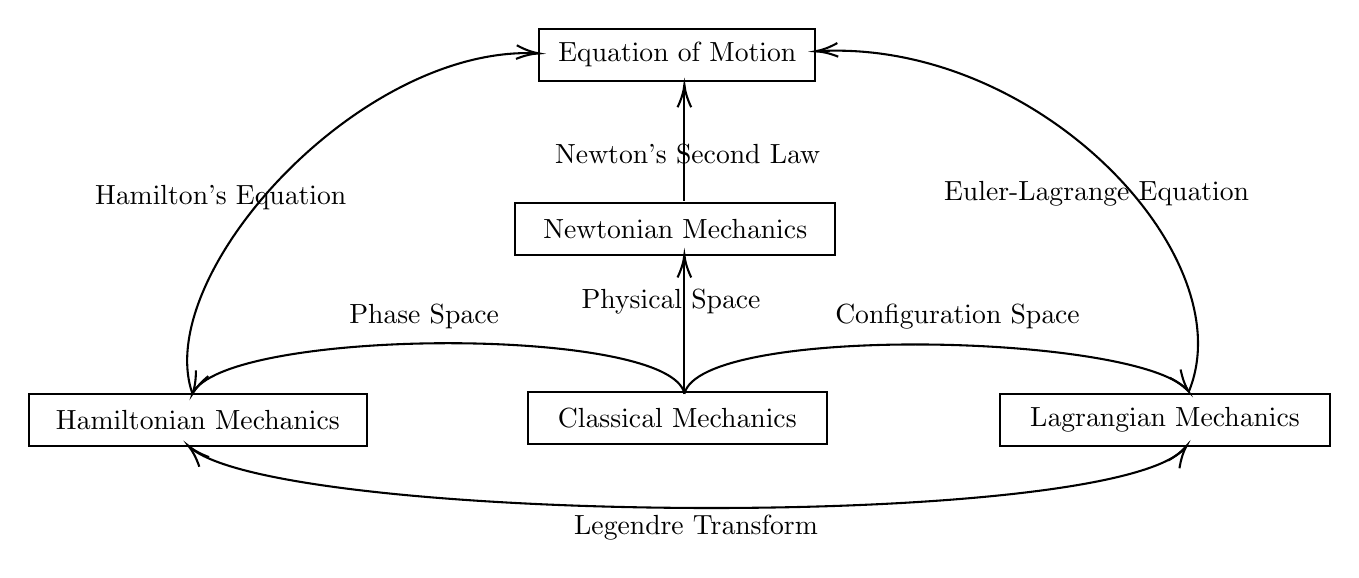
\begin{tikzpicture}[x=0.75pt,y=0.75pt,yscale=-1,xscale=1]
%uncomment if require: \path (0,300); %set diagram left start at 0, and has height of 300

%Straight Lines [id:da6596978253438757] 
\draw    (319.4,108.4) -- (319.4,54.4) ;
\draw [shift={(319.4,52.4)}, rotate = 450] [color={rgb, 255:red, 0; green, 0; blue, 0 }  ][line width=0.75]    (10.93,-3.29) .. controls (6.95,-1.4) and (3.31,-0.3) .. (0,0) .. controls (3.31,0.3) and (6.95,1.4) .. (10.93,3.29)   ;

%Straight Lines [id:da9635704269170282] 
\draw    (319.4,201.4) -- (319.4,136.4) ;
\draw [shift={(319.4,134.4)}, rotate = 450] [color={rgb, 255:red, 0; green, 0; blue, 0 }  ][line width=0.75]    (10.93,-3.29) .. controls (6.95,-1.4) and (3.31,-0.3) .. (0,0) .. controls (3.31,0.3) and (6.95,1.4) .. (10.93,3.29)   ;

%Curve Lines [id:da8601213705090224] 
\draw    (319.4,201.4) .. controls (313.49,168.89) and (103.83,169.38) .. (83.21,199.98) ;
\draw [shift={(82.4,201.4)}, rotate = 295.11] [color={rgb, 255:red, 0; green, 0; blue, 0 }  ][line width=0.75]    (10.93,-3.29) .. controls (6.95,-1.4) and (3.31,-0.3) .. (0,0) .. controls (3.31,0.3) and (6.95,1.4) .. (10.93,3.29)   ;

%Curve Lines [id:da5496082538732877] 
\draw    (319.4,201.4) .. controls (327.28,167.91) and (535.03,172.26) .. (561.33,199.16) ;
\draw [shift={(562.4,200.4)}, rotate = 233.13] [color={rgb, 255:red, 0; green, 0; blue, 0 }  ][line width=0.75]    (10.93,-3.29) .. controls (6.95,-1.4) and (3.31,-0.3) .. (0,0) .. controls (3.31,0.3) and (6.95,1.4) .. (10.93,3.29)   ;

%Curve Lines [id:da6432080478617446] 
\draw    (82.33,228.09) .. controls (129.49,264.15) and (525.01,267.7) .. (560.44,227.63) ;
\draw [shift={(561.4,226.4)}, rotate = 484.44] [color={rgb, 255:red, 0; green, 0; blue, 0 }  ][line width=0.75]    (10.93,-3.29) .. controls (6.95,-1.4) and (3.31,-0.3) .. (0,0) .. controls (3.31,0.3) and (6.95,1.4) .. (10.93,3.29)   ;
\draw [shift={(80.4,226.4)}, rotate = 45.61] [color={rgb, 255:red, 0; green, 0; blue, 0 }  ][line width=0.75]    (10.93,-3.29) .. controls (6.95,-1.4) and (3.31,-0.3) .. (0,0) .. controls (3.31,0.3) and (6.95,1.4) .. (10.93,3.29)   ;
%Curve Lines [id:da7865585332239224] 
\draw    (82.4,201.4) .. controls (62.5,144.68) and (162.39,33.52) .. (248.11,37.33) ;
\draw [shift={(249.4,37.4)}, rotate = 183.33] [color={rgb, 255:red, 0; green, 0; blue, 0 }  ][line width=0.75]    (10.93,-3.29) .. controls (6.95,-1.4) and (3.31,-0.3) .. (0,0) .. controls (3.31,0.3) and (6.95,1.4) .. (10.93,3.29)   ;

%Curve Lines [id:da532295931617982] 
\draw    (562.4,200.4) .. controls (589.26,135.72) and (490.4,30.46) .. (384,36.3) ;
\draw [shift={(382.4,36.4)}, rotate = 356.26] [color={rgb, 255:red, 0; green, 0; blue, 0 }  ][line width=0.75]    (10.93,-3.29) .. controls (6.95,-1.4) and (3.31,-0.3) .. (0,0) .. controls (3.31,0.3) and (6.95,1.4) .. (10.93,3.29)   ;



% Text Node
\draw (325,266) node   [align=left] {Legendre Transform};
% Text Node
\draw (194,164) node   [align=left] {Phase Space};
% Text Node
\draw (451,164) node   [align=left] {Configuration Space};
% Text Node
\draw (313,157) node   [align=left] {Physical Space};
% Text Node
\draw (96,107) node   [align=left] {Hamilton's Equation};
% Text Node
\draw (518,105) node   [align=left] {Euler-Lagrange Equation};
% Text Node
\draw (321,86) node   [align=left] {Newton's Second Law};
% Text Node
\draw    (3.5,201.5) -- (166.5,201.5) -- (166.5,226.5) -- (3.5,226.5) -- cycle  ;
\draw (85,214) node   [align=left] {Hamiltonian Mechanics};
% Text Node
\draw    (244,200.5) -- (388,200.5) -- (388,225.5) -- (244,225.5) -- cycle  ;
\draw (316,213) node   [align=left] {Classical Mechanics};
% Text Node
\draw    (471.5,201.5) -- (630.5,201.5) -- (630.5,226.5) -- (471.5,226.5) -- cycle  ;
\draw (551,214) node   [align=left] {Lagrangian Mechanics};
% Text Node
\draw    (238,109.5) -- (392,109.5) -- (392,134.5) -- (238,134.5) -- cycle  ;
\draw (315,122) node   [align=left] {Newtonian Mechanics};
% Text Node
\draw    (249.5,25.5) -- (382.5,25.5) -- (382.5,50.5) -- (249.5,50.5) -- cycle  ;
\draw (316,38) node   [align=left] {Equation of Motion};


\end{tikzpicture}
\end{center}

\end{qt}


\section{Basic quantities}
\textbf{Momentum} is the velocity of an object times its mass
$$
\vec{p}(t) \equiv m \dot{\vec{q}}(t)
$$
$$
\begin{array}{c}{\frac{d p}{d t}=F} \\ {\int_{t_{i}}^{t_{f}} d p=\int_{t_{i}}^{t_{f}} F d t} \\ {\Delta p=F \Delta t}\end{array}
$$
\textbf{In words, this means that the momentum of an object tells
us how long it takes a given force $F$ to stop it. Formulated
differently, we need a much bigger force to stop it quickly.}

\textbf{Angular momentum} is defined as the cross product of the position vector and the momentum vector
$$
\vec{L}(t)=\vec{q}(t) \times \vec{p}(t)=m \vec{q}(t) \times \dot{q}(t)
$$
While (linear) momentum tells us how hard it
is to stop an object using a specific force, angular momentum tells us how hard it is to stop it spinning.

\textbf{Momentum and angular momentum are conserved.}

\section{Configuration Space}
In a physical space, we use one function $f(x)$ to describe each object in the system separately. In configuration space, we use a vector of functions $\mathbf{r}=[f(x),g(x),h(x)...]$ to describe the system as a whole. \textbf{Using the idea of gluing the
spaces together, we always only need one vector which lives in an an $\mathbb{R}^{N}$ -dimensional space. If the objects are allowed to move freely in three dimensions, our vector $\vec{r}$ lives in $\mathbb{R}^{3 N}$ since we are gluing $ N$ times $\mathbb{R}^{3}$ together.}

In configuration space, we can imagine the whole system as just one point that moves through this higher-dimensional space. Each point in configuration space corresponds to one specific configuration the system can be in.

To summarize: while individual objects move in the three dimensional physical space, the time evolution of a system as a whole takes place in a higher-dimensional configuration space. A single trajectory in configuration space describes the evolution of a system as a whole.

\section{Phase Space}
\textbf{Configuration space only keeps track of the locations of the various objects.} But in addition to a vector that keeps track of the locations, we need a vector that keeps track of the momenta.

This motivates the construction of the  \textbf{phase space} which works completely analogously to how we constructed configuration space. However, this time we also act as if \textbf{the momenta live in a different space and then glue the momentum spaces to our location spaces}. As a result, we can describe the complete state (not just the configuration) of our system with a single vector.
\begin{qt}
\begin{itemize}
    \item Classical mechanics in physical space is what we call the Newtonian formulation.
    \item Classical mechanics in configuration space is what we call the Lagrangian formulation.
    \item Classical mechanics in phase space is what we call the Hamiltonian formulation.
\end{itemize}
\end{qt}


\section{Lagrangian Mechanics}
\begin{quote}
    Any system evolves in such a way that the action required is minimal.
\end{quote}
A path in configuration space between two fixed points $X$ and $Y$ corresponds to one specific possibility for how our system evolves between two fixed configurations. \textbf{We denote the action by $S[q(t)]$ for path the path $q(t)$ from $X$ to $Y$.} And it is calculated as:
$$
\operatorname{action}[q(t)]=S[q(t)]=\int_{t_{i}}^{t_{f}} d t L=\int_{t_{i}}^{t_{f}} d t(T-V)
$$
\subsection{Action and Lagrangian}
\begin{mybox}
why we integrate over $L$ to get the action?
\end{mybox}

\begin{mybox2}
Kinetic energy is a measure for how much is going on in our system.

Potential energy is a measure for how much could happen, but isn’t.

The Lagrangian is therefore a direct measure for the "liveliness" within a system at a specific moment in time. A high kinetic energy implies a large Lagrangian and that our system is extremely lively. A high potential energy implies a small Lagrangian and a less lively system.
\end{mybox2}

\redp{The action $S[q(t)]$ is not a function but a functional.}

\textbf{A function eats a number $x$ and spits out a number $f(x)$. Specifically, the action functional $S[q(t)]$ yields a number for each path $q(t) .$ We call this number the action of the path.}

\redp{The Lagrangian is a function of the location $q$ and the velocity $\frac{d q}{d t}:$ ' $L=L(q, \dot{q}) .$ This means that the Lagrangian does not depend on the
acceleration $\frac{d^{2} q}{d t^{2}}$ or even higher derivatives.}

\subsection{Variational Calculus}
For an ordinary function $f(x),$ we can find the minimum by
calculating the zeroes of its derivative:
$$
\frac{d f(x)}{d x} \stackrel{!}{=} 0
$$

\redp{A minimum is characterized by its neighborhood. If all neighboring points lie higher, the point in question is a minimum.}

\textbf{Let's use this idea to once more find the minimum of the function $f(x)=3 x^{2}+x$.}

We now pick one specific location $x=a$ and start investigating its neighborhood $a \rightarrow a+\epsilon,$ where $\epsilon$ is an infinitesimally small (positive or negative) number. In general, we call $\epsilon$ \textbf{a variation.}

Putting this into the function yields
$$
\begin{aligned} f(a+\epsilon) &=3(a+\epsilon)^{2}+(a+\epsilon) \\ &=3\left(a^{2}+2 a \epsilon+\epsilon^{2}\right)+a+\epsilon \end{aligned}
$$

If the location $a$ is a minimum, we can't get lower by going in any direction $\epsilon .$ Mathematically, this implies: 

\redp{All terms first order in $\epsilon$ must vanish.} Otherwise, for a negative $\epsilon$ the function value $f(a+\epsilon)$ would be smaller than $f(a)$ and therefore, $a$ wouldn't be a minimum.

If we collect all terms linear in $\epsilon$ and demand that they vanish,
$$
\begin{array}{l}{3 \cdot 2 a \epsilon+\epsilon \stackrel{!}{=} 0} \\ {\therefore \quad 6 a+1 \stackrel{!}{=} 0}\end{array}
$$
we find
$$
a=\frac{-1}{6}
$$
The variational method of finding minima can also be applied to functionals like the action $S[q(t)],$ not just functions. Take note that for functionals, our goal isn't to find a location like $a$ which is the minimum of a function but instead, to find a function $q(t)$ which is the minimum of a function.

\subsection{The Euler-Lagrange Equation}
Our task now is to find a method which allows us to calculate
the path $q_m(t)$ for which the action functional is a minimum.

We start again with a concrete choice $q(t)$ and consider small variations around this specific path
\[
q(t) \rightarrow q(t)+\epsilon(t)
\]
$$
\dot{q}(t) \rightarrow \dot{q}(t)+\dot{\epsilon}(t)
$$
where $\epsilon$ is again an infinitesimally small variation.

We consider variations between two fixed configurations $\left(q_{i}\left(t_{i}\right)\right.$ $\left.q_{f}\left(t_{f}\right)\right) .$ Therefore, the variation $\epsilon$ has to vanish at $t_{i}$ and $t_{f}:$
$$
0=\epsilon\left(t_{i}\right)=\epsilon\left(t_{f}\right)
$$
$$
S=\int_{t_{i}}^{t_{f}} d t L(q(t)+\epsilon(t), \dot{q}(t)+\dot{\epsilon}(t))
$$
According to the Taylor expansion,
$$
L(q+\epsilon, \dot{q}+\dot{\epsilon})=L(q, \dot{q})+\epsilon \frac{\partial L}{\partial q}+\dot{\epsilon} \frac{\partial L}{\partial \dot{q}}+\ldots
$$
$$
\begin{aligned}
S &=\int_{t_{i}}^{t_{f}} d t L(a(t)+\epsilon(t), \dot{a}(t)+\dot{\epsilon}(t)) \\
&=\int_{t_{i}}^{t_{f}} d t\left(L(a, \dot{a})+\epsilon \frac{\partial L}{\partial a}+\dot{\epsilon} \frac{\partial L}{\partial \dot{a}}+\ldots\right)
\end{aligned}
$$
\redp{Minima are characterized by vanishing first oerder variations,} so again:
$$
\int_{t_{i}}^{t_{f}} d t\left[\epsilon \frac{\partial L}{\partial q}+\dot{\epsilon} \frac{\partial L}{\partial \dot{q}}\right] \stackrel{!}{=} 0
$$
So, first of all, we integrate by parts the second term on the right-hand side:
$$
\begin{aligned}
\int_{t_{i}}^{t_{f}} d t \dot{\epsilon} \frac{\partial L}{\partial \dot{q}} &=\int_{t_{i}}^{t_{f}} d t\left(\frac{d}{d t} \epsilon\right) \frac{\partial L}{\partial \dot{q}} \\
&=\left.\epsilon \frac{\partial L}{\partial \dot{q}}\right|_{t_{1}} ^{t_{2}}-\int_{t_{i}}^{t_{f}} d t \epsilon \frac{d}{d t}\left(\frac{\partial L}{\partial \dot{q}}\right)
\end{aligned}
$$
since the variation $\epsilon(t)$ vanishes for $t=t_{i}$ and $t=t_{f}$, we have
$$
\begin{aligned}
& \int_{t_{i}}^{t_{f}} d t\left[\epsilon \frac{\partial L}{\partial q}+\dot{\epsilon} \frac{\partial L}{\partial \dot{q}}\right] \stackrel{!}{=} 0 \\
\therefore & \int_{t_{i}}^{t_{f}} d t\left[\epsilon \frac{\partial L}{\partial q}-\epsilon \frac{d}{d t}\left(\frac{\partial L}{\partial \dot{q}}\right)\right] \stackrel{!}{=} 0 \\
\therefore & \int_{t_{i}}^{t_{f}} d t \epsilon\left[\frac{\partial L}{\partial q}-\frac{d}{d t}\left(\frac{\partial L}{\partial \dot{q}}\right)\right] \stackrel{!}{=} 0
\end{aligned}
$$
Now we recall that if $q(t)$ is indeed the path of least action that we are looking for, the condition must be correct for any possible variation $\epsilon=\epsilon(t)$. This can only be correct if:
\begin{qt}
\begin{equation}
\frac{\partial L}{\partial q}-\frac{d}{d t}\left(\frac{\partial L}{\partial \dot{q}}\right) \stackrel{!}{=} 0
\end{equation}
\end{qt}
In particular, for a general potential $V=V(q)$, the first term on LHS yields \textbf{generalized force}:
$$
\frac{\partial L}{\partial q}=\frac{\partial(T(\dot{q})-V(q))}{\partial q}=-\frac{\partial V(q)}{\partial q} \equiv F
$$
In general, the \textbf{conjugate momentum} is:
\begin{equation}
   p \equiv \frac{\partial L}{\partial \dot{q}} 
   \label{conjugate-momentum}
\end{equation}

Therefore, the Euler-Lagrange equation says:
\begin{qt}
\begin{center}
    \textbf{\redp{The rate of change of the momentum equals the force.}}
\end{center}
\end{qt}


In eqn\ref{conjugate-momentum} we call the momentum "\textbf{conjugate momentum}" because it is related to a specific variable $q$. For example, if we describe our system using angles instead of Cartesian coordinates, the corresponding conjugate momenta would be angular momenta.

\section{Hamiltonian Mechanics}
\subsection{Hamilton's Equations}
To derive the equations, the first key idea is that we act as if $q_{i}$ and $p_{i}$ are completely independent variables. We recall the definition of the momentum as:
\begin{equation}
p \equiv \frac{\partial L}{\partial \dot{q}}
\label{ham0}
\end{equation}
According to the Euler-Lagrange equation, we have
\begin{equation}
\frac{d p}{d t}=\frac{\partial L}{\partial q}
\label{ham1}
\end{equation}
Moreover, the definition of the velocity is:
\begin{equation}
\frac{d q}{d t}=\dot{q}
\label{ham2}
\end{equation}
\textbf{Our goal is to rewrite the equations (\ref{ham1}),(\ref{ham2}) in such a way that they only depend on $p$ and no longer on $\dot{q}$.}

First of all we invert eqn(\ref{ham0}) to get $\dot{q}=\dot{q}(q, p)$, from which we get new function:
\begin{equation}
    \tilde{L}(q, p) \equiv L(q, \dot{q}(q, p))
\end{equation}
In words, $\tilde{L}(q, p)$ is the function that we get if we use the formula $\dot{q}=\dot{q}(q, p)$ to eliminate $\dot{q}$ from $L(q, \dot{q}) .$ In particular, take note that, in general,
\begin{equation}
\tilde{L}(q, p) \neq L(q, p)
\end{equation}
For example, for the free Lagrangian
$$
\begin{aligned}
\tilde{L}(q, p) & \stackrel{(1.6)}{=} L(q, \dot{q}(q, p)) \\
&=\frac{m(\dot{q}(q, p))^{2}}{2} \\
&=\frac{m\left(\frac{p}{m}\right)^{2}}{2} \\
&=\frac{p^{2}}{2 m}
\end{aligned}
$$
Therefore
$$
L(q, p)=\frac{m p^{2}}{2} \neq \frac{p^{2}}{2 m}=\tilde{L}(q, p)
$$
Now when we calculate the derivative, we find:
$$
\begin{aligned}
&\frac{\partial \tilde{L}(q, p)}{\partial q} \stackrel{(1.6)}{=} \frac{\partial L(q, \dot{q}(q, p))}{\partial q}\\
&\frac{\partial \tilde{L}(q, p)}{\partial q}=\frac{\partial L(q, \dot{q})}{\partial q}+\frac{\partial L(q, \dot{q})}{\partial \dot{q}} \frac{\partial \dot{q}(q, p)}{\partial q}\\
&\frac{\partial \tilde{L}(q, p)}{\partial q}=\frac{\partial L(q, \dot{q})}{\partial q}+p \frac{\partial \dot{q}(q, p)}{\partial q}
\end{aligned}
$$
Since $\frac{\partial}{\partial q} p q=p \frac{\partial}{\partial q} q$ because $\frac{\partial}{\partial q} p=0$, we have
$$
\begin{aligned}
&\frac{\partial L(q, \dot{q})}{\partial q}=\frac{\partial \tilde{L}(q, p)}{\partial q}-p \frac{\partial \dot{q}(q, p)}{\partial q}\\
&\frac{\partial L(q, \dot{q})}{\partial q}=\frac{\partial}{\partial q}(\tilde{L}(q, p)-p \dot{q}(q, p))
\end{aligned}
$$
From eqn.(\ref{ham1}), we have
\begin{equation}
\begin{aligned}
\frac{d p}{d t} &=\frac{\partial L}{\partial q} \\
&=\frac{\partial}{\partial q}(L(q, p)-p \dot{q}(q, p)) \\
&=-\frac{\partial H}{\partial q}
\end{aligned}
\end{equation}
where we define \textbf{the Hamiltonian as}
\begin{equation}
H \equiv p \dot{q}(q, p)-\tilde{L}(q, p)
\end{equation}
Similarly, we calculate the derivative of $\tilde{L}(q,p)$ with respect to $p$:
$$
\begin{aligned}
&\frac{\partial \tilde{L}(q, p)}{\partial p} \stackrel{(1.6)}{=} \frac{\partial L(q, \dot{q}(q, p))}{\partial p}\\
&\frac{\partial \tilde{L}(q, p)}{\partial p}=\frac{\partial L(q, \dot{q})}{\partial \dot{q}} \frac{\partial \dot{q}}{\partial p}\\
&\frac{\partial \tilde{L}(q, p)}{\partial p}=p \frac{\partial \dot{q}}{\partial p}\\
&\frac{\partial \tilde{L}(q, p)}{\partial p}=\frac{\partial}{\partial p}(p \dot{q})-\dot{q}
\end{aligned}
$$
Rearrange terms, we obtain
\begin{equation}
\frac{\partial H}{\partial p}=\dot{q}
\end{equation}
In summary, the \textbf{Hamilton's equations} are simply:
\begin{equation}
\begin{aligned}
&\frac{d p}{d t}=-\frac{\partial H}{\partial q}\\
&\frac{d q}{d t}=\frac{\partial H}{\partial p}
\end{aligned}
\end{equation}
As before, if there are multiple objects in the system moving in three dimensions, we need to take all their locations and momenta into account. Hamilton's equations then read
\begin{equation}
\begin{aligned}
&\frac{d p_{i}}{d t}=-\frac{\partial H}{\partial q_{i}}\\
&\frac{d q_{i}}{d t}=\frac{\partial H}{\partial p_{i}}
\end{aligned}
\end{equation}

\subsection{Alternative way to derive Hamilton's equation}
From the definition of action and Hamilton, we have:
$$
\begin{aligned}
S &=\int_{t_{\mathrm{i}}}^{t} d t L \\
&=\int_{t_{\mathrm{i}}}^{t} d t(p \dot{q}-H)
\end{aligned}
$$
Now we can once more use the least action princople to derive the correct equations of motion. \textbf{We are searching a path in phase space that minimize the $S$}:
$$
\begin{aligned}
&S=\int_{t_{i}}^{t_{f}} d t(p \dot{q}-H(q, p))=\int_{t_{i}}^{t_{f}} d t\left(p \frac{d}{d t} q-H(q, p)\right)\\
&S=\int_{t_{i}}^{t_{f}} d t\left(((p+\tilde{\epsilon})) \frac{d}{d t}(q+\epsilon)-H(q+\epsilon, p+\tilde{\epsilon})\right)
\end{aligned}
$$
$$
\begin{aligned}
=\int_{t_{\mathrm{i}}}^{t_{f}} d t &\left((p+\tilde{\epsilon}) \frac{d}{d t}(q+\epsilon)\right.\\
&\left.-H(q, p)-\epsilon \frac{\partial H(q, p)}{\partial q}-\tilde{\epsilon} \frac{\partial H(q, p)}{\partial p}-\cdots\right) \\
=\int_{t_{\mathrm{i}}}^{t_{\mathrm{f}}} d t &\left(p \frac{d q}{d t}-H+\tilde{\epsilon}\left(\frac{d}{d t} q-\frac{\partial H}{\partial p}\right)+\ldots\right.\\
&\left.-\epsilon \frac{\partial H}{\partial q}+p \frac{d \epsilon}{d t}+\tilde{\epsilon} \frac{d \epsilon}{d t}\right)
\end{aligned}
$$
In the last line we have a term proportional to $\frac{d\epsilon}{dt}$, but we can turn it into a term proportional to $\epsilon$ by integrating by parts:
$$
\begin{aligned}
\int_{t_{\mathrm{i}}}^{t_{f}} d t p \frac{d \epsilon}{d t} &=\left.\epsilon p\right|_{t_{\mathrm{i}}} ^{t_{f}}-\int_{t_{\mathrm{i}}}^{t_{f}} d t \frac{d p}{d t} \epsilon \\
&=-\int_{t_{\mathrm{i}}}^{t_{f}} d t \frac{d p}{d t} \epsilon
\end{aligned}
$$
because $\epsilon\left(t_{i}\right)=\epsilon\left(t_{f}\right)=0$. By using this, we can factor out $\epsilon$:
$$
\begin{aligned}
S=\int_{t_{i}}^{t_{f}} d t &\left(p \frac{d q}{d t}-H+\tilde{\epsilon}\left(\frac{d}{d t} q-\frac{\partial H}{\partial p}\right)+\ldots\right.\\
&\left.-\epsilon \frac{\partial H}{\partial q}+p \frac{d \epsilon}{d t}+\tilde{\epsilon} \frac{d \epsilon}{d t}\right)
\end{aligned}
$$
$$
\begin{aligned}
=\int_{t_{\mathrm{i}}}^{t} d t &\left(p \frac{d q}{d t}-H+\tilde{\epsilon}\left(\frac{d}{d t} q-\frac{\partial H}{\partial p}\right)+\ldots\right.\\
&\left.-\epsilon \frac{\partial H}{\partial q}-\frac{d p}{d t} \epsilon+\tilde{\epsilon} \frac{d \epsilon}{d t}\right) \\
=\int_{t_{\mathrm{i}}}^{t} d t &\left(p \frac{d q}{d t}-H+\tilde{\epsilon}\left(\frac{d}{d t} q-\frac{\partial H}{\partial p}\right)+\ldots\right.\\
&\left.-\epsilon\left(\frac{\partial H}{\partial q}+\frac{d p}{d t}\right)+\tilde{\epsilon} \frac{d \epsilon}{d t}\right)
\end{aligned}
$$
This means that the terms linear in $\epsilon$ and $\tilde{\epsilon}$ only vanish, in general, if the following two conditions are fulfilled:
\begin{equation}
\begin{aligned}
&\frac{\partial H}{\partial q}+\frac{d}{d t} p \stackrel{!}{=} 0\\
&\frac{\partial H}{\partial p}-\frac{d}{d t} q \stackrel{!}{=} 0
\end{aligned}
\end{equation}
The path $(q(t), p(t))$ which fulfills these two conditions is the correct path which minimizes the action and therefore describes the evolution of our system.

The following diagram illustrates the relationship between the derivations discussed above:
\begin{qt}
\begin{center}
    


\tikzset{every picture/.style={line width=0.75pt}} %set default line width to 0.75pt        

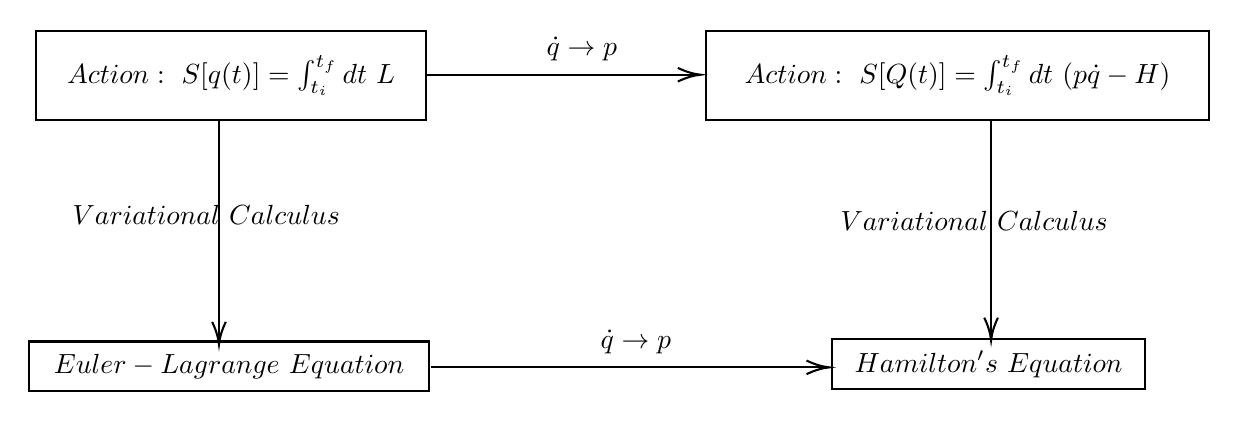
\begin{tikzpicture}[x=0.75pt,y=0.75pt,yscale=-1,xscale=1]
%uncomment if require: \path (0,300); %set diagram left start at 0, and has height of 300

%Straight Lines [id:da8998412978689948] 
\draw    (199.17,49.47) -- (329.17,49.47) ;
\draw [shift={(331.17,49.47)}, rotate = 180] [color={rgb, 255:red, 0; green, 0; blue, 0 }  ][line width=0.75]    (10.93,-3.29) .. controls (6.95,-1.4) and (3.31,-0.3) .. (0,0) .. controls (3.31,0.3) and (6.95,1.4) .. (10.93,3.29)   ;

%Straight Lines [id:da28118020162887525] 
\draw    (99.17,71.47) -- (99.17,177.47) ;
\draw [shift={(99.17,179.47)}, rotate = 270] [color={rgb, 255:red, 0; green, 0; blue, 0 }  ][line width=0.75]    (10.93,-3.29) .. controls (6.95,-1.4) and (3.31,-0.3) .. (0,0) .. controls (3.31,0.3) and (6.95,1.4) .. (10.93,3.29)   ;

%Straight Lines [id:da2698264444244326] 
\draw    (201.17,190.47) -- (391.17,190.47) ;
\draw [shift={(393.17,190.47)}, rotate = 180] [color={rgb, 255:red, 0; green, 0; blue, 0 }  ][line width=0.75]    (10.93,-3.29) .. controls (6.95,-1.4) and (3.31,-0.3) .. (0,0) .. controls (3.31,0.3) and (6.95,1.4) .. (10.93,3.29)   ;

%Straight Lines [id:da134942784322725] 
\draw    (471.17,71.47) -- (471.17,175.47) ;
\draw [shift={(471.17,177.47)}, rotate = 270] [color={rgb, 255:red, 0; green, 0; blue, 0 }  ][line width=0.75]    (10.93,-3.29) .. controls (6.95,-1.4) and (3.31,-0.3) .. (0,0) .. controls (3.31,0.3) and (6.95,1.4) .. (10.93,3.29)   ;


% Text Node
\draw    (11,28.5) -- (199,28.5) -- (199,71.5) -- (11,71.5) -- cycle  ;
\draw (105,50) node    {$Action:\ S[ q( t)] =\int ^{t_{f}}_{t_{i}} dt\ L$};
% Text Node
\draw (274,37) node    {$\dot{q}\rightarrow p$};
% Text Node
\draw    (334,28.5) -- (576,28.5) -- (576,71.5) -- (334,71.5) -- cycle  ;
\draw (455,50) node    {$Action:\ S[ Q( t)] =\int ^{t_{f}}_{t_{i}} dt\ ( p\dot{q} -H)$};
% Text Node
\draw    (7.5,178) -- (200.5,178) -- (200.5,202) -- (7.5,202) -- cycle  ;
\draw (104,190) node    {$Euler-Lagrange\ Equation$};
% Text Node
\draw    (394.5,177) -- (545.5,177) -- (545.5,201) -- (394.5,201) -- cycle  ;
\draw (470,189) node    {$Hamilton's\ Equation$};
% Text Node
\draw (93,117) node    {$Variational\ Calculus$};
% Text Node
\draw (300,178) node    {$\dot{q}\rightarrow p$};
% Text Node
\draw (463,120) node    {$Variational\ Calculus$};


\end{tikzpicture}

\end{center}
\end{qt}


\subsection{Meaning of Hamilton's Equation}
First of all, \textbf{we need to calculate the momentum explicitly:}
$$
\begin{aligned}
p & \equiv \frac{\partial L}{\partial \dot{q}} \\
&=\frac{\partial\left(\frac{1}{2} m \dot{q}^{2}-V(q)\right)}{\partial \dot{q}} \\
&=m \dot{q}
\end{aligned}
$$
Using this result, we ca derive the Hamiltonian:
$$
\begin{aligned}
H &=p \dot{q}-L \\
&=p \dot{q}-\left(\frac{1}{2} m \dot{q}^{2}-V(q)\right) \\
&=p \frac{p}{m}-\left(\frac{1}{2} m\left(\frac{p}{m}\right)^{2}-V(q)\right) \\
&=\frac{p^{2}}{2 m}+V(q)
\end{aligned}
$$
This is exactly the total energy of the object.\redp{The Hamiltonian represents the total energy.}

From the first Hamilton's equation, we have
$$
\begin{aligned}
\frac{d p}{d t} &=-\frac{\partial H}{\partial q} \\
&=-\frac{\partial\left(\frac{p^{2}}{2 m}+V(q)\right)}{\partial q} \\
&=-\frac{\partial V(q)}{\partial q}
\end{aligned}
$$
That is, \redp{The rate of change of momentum equals the force}.

Hamilton's second equation reads:
$$
\begin{aligned}
\frac{d q}{d t} &=\frac{\partial H}{\partial p} \\
&=\frac{\partial\left(\frac{1}{2} \frac{p^{2}}{m}+V(q)\right)}{\partial p} \\
&=\frac{p}{m}
\end{aligned}
$$
Therefore, we can now understand that \redp{the purpose of Hamilton’s second law is to establish a relationship between the momentum and the rate of change of the position}.

\subsection{Hamilton's General Equation}
First of all, we can imagine that sometimes we are not only interested in the locations and momenta of the various objects in
the system but other quantities too. For instance, the temperature or how the kinetic energy evolves as time passes can be interesting things to investigate. \redp{In phase space, the quantities like the temperature or kinetic energy are functions of $q_i$ and $p_i$.}

\begin{mybox}
But how can we calculate the time evolution of such functions depending on the locations $q_{i}(t)$ and momenta $p_{i}(t) ?$
\end{mybox}
For simplicity, let's restrict ourselves to one object moving in one dimension. Then the total rate of change of a function $F=$ $F(q(t), p(t))$ along a single object's trajectory reads:
$$
\frac{d}{d t} F(q, p)=\frac{\partial F(q, p)}{\partial q} \frac{d q}{d t}+\frac{\partial F(q, p)}{\partial p} \frac{d p}{d t}
$$
Using Hamilton's equations, we can write:
$$
\begin{aligned}
\frac{d}{d t} F(q, p) &=\frac{\partial F(q, p)}{\partial q} \frac{d q}{d t}+\frac{\partial F(q, p)}{\partial p} \frac{d p}{d t} \\
&=\frac{\partial F(q, p)}{\partial q} \frac{\partial H(q, p)}{\partial p}-\frac{\partial F(q, p)}{\partial p} \frac{\partial H(q, p)}{\partial q}
\end{aligned}
$$
since the structure that appears on the right-hand side here is so important, it is conventional to introduce a more compact notation. We therefore introduce the \textbf{Poisson bracket $\{,\}$ of two phase space functions $A(q, p), B(q, p)$ by defining}:
\begin{qt}
    \begin{equation}
        \{A, B\} \equiv \frac{\partial A}{\partial q} \frac{\partial B}{\partial p}-\frac{\partial A}{\partial p} \frac{\partial B}{\partial q}
    \end{equation}
\end{qt}
This means that you can’t combine two functions in phase space which describe properties of our system arbitrarily and expect to get something that describes another useful property of
the system. But \textbf{if you calculate the Poisson bracket of the two functions, you’ll get something sensible.} 

Thus, the equation
\begin{qt}
    \begin{equation}
\frac{d}{d t} F=\{F, H\}
\end{equation}
\end{qt}
describes the time evolution of a general phase spack function and we call it \textbf{Hamilton's equation of motion.}

Notice that
\begin{qt}
    $$
\begin{aligned}
\frac{d}{d t} q &=\{q, H\} \\
&=\frac{\partial q}{\partial q} \frac{\partial H}{\partial p}-\frac{\partial q}{\partial p} \frac{\partial H}{\partial q} \\
&=\frac{\partial H}{\partial p}
\end{aligned}
$$
\end{qt}
and
\begin{qt}
    $$
\begin{aligned}
\frac{d}{d t} p &=\{p, H\} \\
&=\frac{\partial p}{\partial q} \frac{\partial H}{\partial p}-\frac{\partial p}{\partial p} \frac{\partial H}{\partial q} \\
&=-\frac{\partial H}{\partial q}
\end{aligned}
$$
\end{qt}
\redp{\textbf{So one way to understand Hamilton's general equation of motion is by imagining that we have a new kind of object $\{, H\}$ (an operator) which eats any function $F$ on phase space $(\{F, H\})$ and spits out the correct time evolution of $F$.}}
\begin{qt}
\begin{center}
    \textbf{The Hamiltonian generates time evolution in phase space.}
\end{center}
\end{qt}
Sometimes we are déaling with a function in phase space which not only depends on $q$ and $p,$ but also explicitly on $t .$ For example, this is necessarily the case if there is a time-dependent potential $V=V(q, t) .$ The total rate of change then reads:
\begin{equation}
\frac{d}{d t} F(q, p, t)=\frac{d q}{d t} \frac{\partial F}{\partial q}+\frac{d p}{d t} \frac{\partial F}{\partial p}+\frac{\partial F}{\partial t}
\end{equation}
In other words,
\begin{qt}
\begin{equation}
\frac{d}{d t} F(q, p, t)=\{F, H\}+\frac{\partial F}{\partial t}
\end{equation}
\end{qt}

\section{The Newtonian Algorithm}
\begin{mybox}
We stand at the top of the Leaning Tower of Pisa and let a ball fall to the ground. How is the ball moving?
\end{mybox}
$$
\vec{F}=\left(\begin{array}{r}
{0} \\
{0} \\
{-m g}
\end{array}\right)
$$
Newton's second law tells us
$$
\begin{aligned}
\frac{d \vec{p}}{d t} &=\vec{F} \\
\frac{d(m \vec{v})}{d t} &=\left(\begin{array}{r}
{0} \\
{0} \\
{-m g}
\end{array}\right) \\
m \frac{d}{d t}\left(\begin{array}{l}
{v_{x}} \\
{v_{z}}
\end{array}\right) &=\left(\begin{array}{r}
{0} \\
{-m g}
\end{array}\right) \\
\frac{d}{d t}\left(\begin{array}{l}
{v_{x}} \\
{v_{z}}
\end{array}\right) &=\left(\begin{array}{r}
{0} \\
{-g}
\end{array}\right)
\end{aligned}
$$
Our task is to solve these three equations of motion. Luckily, we can simply integrate the equations twice since gravity is constant:
$$
\begin{aligned}
\frac{d}{d t}\left(\begin{array}{c}
{v_{x}} \\
{v_{y}} \\
{v_{z}}
\end{array}\right) &=\left(\begin{array}{c}
{0} \\
{0} \\
{-g}
\end{array}\right) \\
\int_{0}^{t} d t^{\prime} \frac{d}{d t^{\prime}}\left(\begin{array}{c}
{v_{x}} \\
{v_{y}} \\
{v_{z}}
\end{array}\right) &=\int_{0}^{t} d t^{\prime}\left(\begin{array}{c}
{0} \\
{-g}
\end{array}\right) \\
\left(\begin{array}{c}
{v_{x}(t)} \\
{v_{z}(t)}
\end{array}\right)-\left(\begin{array}{c}
{v_{x}(0)} \\
{v_{z}(0)}
\end{array}\right)=\left(\begin{array}{c}
{0} \\
{0} \\
{-g t}
\end{array}\right)
\end{aligned}
$$
$\int_{0}^{t} d t^{\prime}\left(\begin{array}{l}{v_{x}\left(t^{\prime}\right)} \\ {v_{y}\left(t^{\prime}\right)} \\ {v_{z}\left(t^{\prime}\right)}\end{array}\right)-\int_{0}^{t} d t^{\prime}\left(\begin{array}{l}{v_{x}(0)} \\ {v_{y}(0)} \\ {v_{z}(0)}\end{array}\right)=\int_{0}^{t} d t^{\prime}\left(\begin{array}{c}{0} \\ {0} \\ {-g t}\end{array}\right)$
$$
\left(\begin{array}{l}
{x(t)} \\
{y(t)} \\
{z(t)}
\end{array}\right)-\left(\begin{array}{l}
{x(0)} \\
{y(0)} \\
{z(0)}
\end{array}\right)-\left(\begin{array}{l}
{v_{x}(0) t} \\
{v_{y}(0) t} \\
{v_{z}(0) t}
\end{array}\right)=\left(\begin{array}{c}
{0} \\
{0} \\
{-\frac{1}{2} g t^{2}}
\end{array}\right)
$$
Next, we need to determine the integration constants
$$
v_{x}(0), v_{y}(0), v_{z}(0), x(0), y(0), z(0)
$$
Let
$$
\left(\begin{array}{l}
{v_{x}(0)} \\
{v_{y}(0)} \\
{v_{z}(0)}
\end{array}\right)=\left(\begin{array}{l}
{0} \\
{0} \\
{0}
\end{array}\right)
$$
$$
\left(\begin{array}{l}
{x(0)} \\
{y(0)} \\
{z(0)}
\end{array}\right)=\left(\begin{array}{l}
{0} \\
{0} \\
{0}
\end{array}\right)
$$
Finally
$$
\left(\begin{array}{c}
{x(t)} \\
{y(t)} \\
{z(t)}
\end{array}\right)=\left(\begin{array}{c}
{0} \\
{0} \\
{-\frac{1}{2} g t^{2}}
\end{array}\right)
$$
\section{Lagrangian Algorithm}
\begin{mybox}
We stand at the top of the Leaning Tower of Pisa and let a ball fall to the ground. How is the ball moving?
\end{mybox}
The Lagrangian reads
$$
\begin{aligned}
L=T-V &=\frac{1}{2} m \vec{v}^{2}-m g z \\
&=\frac{1}{2} m\left(v_{x}^{2}+v_{y}^{2}+v_{z}^{2}\right)-m g z
\end{aligned}
$$
Since $\frac{\partial L}{\partial q}=\frac{d}{d t}\left(\frac{\partial L}{\partial v_{q}}\right)$,
$$
0=m \frac{d}{d t} v_{x}
$$
$$
0=m \frac{d}{d t} v_{y}
$$
$$
-m g=m \frac{d}{d t} v_{z}
$$
\textbf{Take note that in the derivations above, we didn’t have to think about vectors at all. This is one advantage of the Lagrangian formalism.} In addition, the Lagrangian formulation of classical mechanics is always a good choice whenever we are dealing with a system which is subject to constraints.

\subsection{Constraints}
In mathematical terms, a constraint is a relationship between coordinates. For example, for a mass attached to a circular loop with radius $l,$ we have the constraint
$$
x^{2}+y^{2}=l^{2}
$$
More generally, a \textbf{holonomic constraint} is a formula of the form
$$
f\left(q, 1, q_{2}, \ldots, t\right)=\text { const. }
$$
\begin{qt}
\textbf{Non-holonomic constraints}
$$
f\left(q_{1}, 1, q_{2}, \ldots\right) \geq \text { const. }
$$
$$
f(q, \dot{q}, t)=\text { const. }
$$
Additionally, take note that it is conventional to call a constraint which does not explicitly depend on $t$ scleronomic (Greek for "rigid") and a constraint with explicit dependence on $t$ rheonomic (Greek for "moving").
\end{qt}
The trick which allows us to incorporate constraints in the Lagrangian formalism is known as the method of \textbf{Lagrange multipliers} and works as follows.
\begin{mybox}
\begin{center}
    How to use Lagrange multiplier to add a holonomic constraint?
\end{center}
\end{mybox}
\begin{mybox2}
First, we rewrite the constraint as:
$$
g\left(q_{1}, 1, q_{2}, \ldots, t\right) \equiv f\left(q_{1}, 1, q_{2}, \ldots, t\right)-\text { const. }
$$
We then take the Lagrangian $L_{\text {free that we would use if the }}$ object could move around freely without constraints and add a new term $L_{\text {con}}$  which encodes the constraint 
$$
\begin{aligned}
L_{\text {full }} &=L_{\text {free }}+L_{\text {con }} \\
&=L_{\text {free }}+\lambda g(q, t)
\end{aligned}
$$
If we treat $\lambda$ as a new coordinate, the Euler-Lagrange equation for $\lambda$ tells us
$$
\begin{array}{c}
{\frac{\partial L}{\partial \lambda}=\frac{d}{d t}\left(\frac{\partial L}{\partial \dot{\lambda}}\right)} \\
{\frac{\partial\left(L_{\text {free }}+\lambda g(q, t)\right)}{\partial \lambda}=\frac{d}{d t}\left(\frac{\partial\left(L_{\text {free }}+\lambda g(q, t)\right)}{\partial \lambda}\right)} \\
{\frac{\partial(\lambda g(q, t))}{\partial \lambda}=\frac{d}{d t}\left(\frac{\partial(\lambda g(q, t))}{\partial \dot{\lambda}}\right)} \\
{\frac{\partial(\lambda g(q, t))}{\partial \lambda}=0} \\
{g(q, t)=0}
\end{array}
$$
In addition, by using the Euler-Lagrange equation for our ordinary coordinates $q,$ we find
$$
\begin{aligned}
\frac{\partial L}{\partial q} &=\frac{d}{d t}\left(\frac{\partial L}{\partial \dot{q}}\right) \\
\frac{\partial\left(L_{\text {free }}+\lambda g(q, t)\right)}{\partial q} &=\frac{d}{d t}\left(\frac{\partial\left(L_{\text {free }}+\lambda g(q, t)\right)}{\partial \dot{q}}\right) \\
\frac{\partial\left(L_{\text {free }}+\lambda g(q, t)\right)}{\partial q} &=\frac{d}{d t}\left(\frac{\partial L_{\text {free }}}{\partial \dot{q}}\right) \\
\frac{\partial L_{\text {free }}}{\partial q}+\lambda \frac{\partial g(q, t)}{\partial q} &=\frac{d}{d t}\left(\frac{\partial L_{\text {free }}}{\partial \dot{q}}\right)
\end{aligned}
$$
we've learned that the term on the right-hand side $\frac{d}{d t}\left(\frac{\partial L_{\text {free }}}{\partial q}\right)$ is analogous to $\frac{d p}{d t}$ in the Newtonian formalism. Moreover, the first term on the left-hand side $\frac{\partial L_{\text {free }}}{\partial q}$ describes the forces. In other words, $\lambda \frac{\partial g(q, t)}{\partial q}$ add new forces to the equation of motion.
\end{mybox2}
If there is more than one constraint
$$
L_{\text {full }}=L_{\text {free }}+\lambda_{1 g_{1}}(q, t)+\lambda_{2} g_{1}(q, t)+\ldots
$$
Moreover, using the Euler-Lagrange equation for the regular coordinate $q$ yields the equation of motion including all constraint forces:
$$
\frac{\partial L_{\text {free }}}{\partial q}+\lambda_{1} \frac{\partial g_{1}(q, t)}{\partial q}+\lambda_{2} \frac{\partial g_{2}(q, t)}{\partial q}+\ldots=\frac{d}{d t}\left(\frac{\partial L_{\text {free }}}{\partial \dot{q}}\right)
$$

\subsection{Point Transformations and Generalized Coordinates}
In general, we call a transformation from one set of coordinates in configuration space $q=\left(q_{1}, q_{2}, \ldots\right)$ to a new set of coordinates $q^{\prime}=\left(q_{1}^{\prime}, q_{2}^{\prime}, \ldots\right)$ a\textbf{ point transformation.}
\begin{qt}
\begin{center}
    The Euler-Lagrange equation is valid for any choice of coordinates.
\end{center}
\end{qt}
It is conventional to rephrase this by saying that in the Lagrangian formalism, we are free to use generalized coordinates. Formulated differently, if we find such coordinates for which the constraint term vanishes, we’ve found the most natural coordinates to describe our system.
\begin{mybox}
\begin{center}
    Now, why does the Euler-Lagrange equation look exactly the same no matter which coordinates we choose?
\end{center}
\end{mybox}
\begin{mybox2}
We want to show that no matter which transformation formulas we use
$$
\begin{aligned}
&q^{\prime}=q^{\prime}(q, t)\\
&\dot{q}^{\prime}=\dot{q}^{\prime}(q, \dot{q}, t)
\end{aligned}
$$
the Euler-Lagrange equation in terms of the new coordinates
$$
\frac{\partial \tilde{L}}{\partial q^{\prime}}-\frac{d}{d t}\left(\frac{\partial \tilde{L}}{\partial \dot{q}^{\prime}}\right)=0
$$
where
$$
L\left(q^{\prime}, \dot{q}^{\prime}, t\right)=L\left(q\left(q^{\prime}, t\right), \dot{q}\left(q^{\prime}, \dot{q}^{\prime}, t\right), t\right)
$$
also
$$
\begin{aligned}
\dot{q} &=\frac{d}{d t} q\left(q^{\prime}, t\right) \\
&=\frac{\partial q}{\partial q^{\prime}} \frac{d q^{\prime}}{d t}+\frac{\partial q}{\partial t} \\
&=\frac{\partial q}{\partial q^{\prime}} \dot{q}^{\prime}+\frac{\partial q}{\partial t}
\end{aligned}
$$
which implies
$$
\begin{aligned}
\frac{\partial}{\partial \dot{q}^{\prime}} \dot{q}= & \frac{\partial}{\partial \dot{q}^{\prime}}\left(\frac{\partial q}{\partial q^{\prime}} \dot{q}^{\prime}+\frac{\partial q}{\partial t}\right) \\
&=\frac{\partial q}{\partial q^{\prime}}
\end{aligned}
$$
Secondly
$$
\begin{aligned}
\frac{\partial \tilde{L}}{\partial q^{\prime}} &=\frac{\partial L\left(q\left(q^{\prime}, t\right), \dot{q}\left(q^{\prime}, \dot{q}^{\prime}, t\right), t\right)}{\partial q^{\prime}} \\
&=\frac{\partial L}{\partial q} \frac{\partial q}{\partial q^{\prime}}+\frac{\partial L}{\partial \dot{q}} \frac{\partial \dot{q}}{\partial q^{\prime}}
\end{aligned}
$$
Thirdly
$$
\begin{aligned}
\frac{\partial \tilde{L}}{\partial \dot{q}^{\prime}} & = \frac{\partial L\left(q\left(q^{\prime}, t\right), \dot{q}\left(q^{\prime}, \dot{q}^{\prime}, t\right), t\right)}{\partial \dot{q}^{\prime}} \\
&=\frac{\partial L}{\partial \dot{q}} \frac{\partial \dot{q}^{\prime}}{\partial \dot{q}^{\prime}} \\
&=\frac{\partial L}{\partial \dot{q}} \frac{\partial q}{\partial q^{\prime}}
\end{aligned}
$$
which implies
$$
\begin{aligned}
\frac{d}{d t} \frac{\partial \tilde{L}}{\partial \dot{q}^{\prime}} &= \frac{d}{d t}\left(\frac{\partial L}{\partial \dot{q}} \frac{\partial q}{\partial q^{\prime}}\right) \\
&=\left(\frac{d}{d t} \frac{\partial L}{\partial \dot{q}}\right) \frac{\partial q}{\partial q^{\prime}}+\frac{\partial L}{\partial \dot{q}}\left(\frac{d}{d t} \frac{\partial q}{\partial q^{\prime}}\right) \\
&=\left(\frac{d}{d t} \frac{\partial L}{\partial \dot{q}}\right) \frac{\partial q}{\partial q^{\prime}}+\frac{\partial L}{\partial \dot{q}} \frac{\partial \dot{q}}{\partial q^{\prime}}
\end{aligned}
$$
\end{mybox2}
\begin{mybox2}
With these formulas at hand, let’s rewrite the "new" Euler-Lagrange equation
$$
0 \stackrel{!}{=} \frac{\partial \tilde{L}}{\partial q^{\prime}}-\frac{d}{d t}\left(\frac{\partial \tilde{L}}{\partial \dot{q}^{\prime}}\right)
$$
$$
\begin{aligned}
&=\left(\frac{\partial L}{\partial q} \frac{\partial q}{\partial q^{\prime}}+\frac{\partial L}{\partial \dot{q}} \frac{\partial \dot{q}}{\partial q^{\prime}}\right)-\left(\left(\frac{d}{d t} \frac{\partial L}{\partial \dot{q}}\right) \frac{\partial q}{\partial q^{\prime}}+\frac{\partial L}{\partial \dot{q}} \frac{\partial \dot{q}}{\partial q^{\prime}}\right)\\
&=\frac{\partial L}{\partial q} \frac{\partial q}{\partial q^{\prime}}-\left(\frac{d}{d t} \frac{\partial L}{\partial \dot{q}}\right) \frac{\partial q}{\partial q^{\prime}}\\
&=\left(\frac{\partial L}{\partial q}-\frac{d}{d t} \frac{\partial L}{\partial \dot{q}}\right) \frac{\partial q}{\partial q^{\prime}}=0
\end{aligned}
$$
\end{mybox2}

However, take note that we’ve only shown that the Euler-Lagrange equation has the same form no matter which coordinates we use. In technical terms,\textbf{ we say the Euler-Lagrange equation is only covariant but not invariant under general coordinate transformations.}


\subsection{Gauge Transformation}
We can not only change our configuration space coordinates $q,$ but we can also change the Lagrangian itself and consequently also the action itself without changing the Euler-Lagrange equations.This is possible because \textbf{the number which the action functional $S[q(t)]$ assigns to each path $q(t)$ is not really important. Instead, \bluep{the only thing we really care about is the relative difference between the numbers assigned to different paths}.}

In particular, the Euler-Lagrange equation does not change when we add the total time derivative of any (differentiable) function $F$ which only depends on the location $q$ and possibly the time coordinate $t$ to the Lagrangian
\begin{qt}
\begin{equation}
L \rightarrow L^{\prime}=L+\frac{d F(q, t)}{d t}
\end{equation}
\end{qt}
We call this kind of transformation a \textbf{gauge transformation}.
Now the "new" action can be calculated as:
$$
\begin{aligned}
S^{\prime}[q(t)] &=\int_{t_{i}}^{t_{f}} d t L^{\prime}(q(t), \dot{q}(t), t) \\
&=\int_{t_{i}}^{t_{f}} d t(L(q(t), \dot{q}(t), t)+F(q(t), t))
\end{aligned}
$$
$$
\begin{aligned}
&=\left(\int_{t_{i}}^{t_{f}} d t L\right)+F\left(q\left(t_{f}\right), t_{f}\right)-F\left(q\left(t_{i}\right), t_{i}\right)\\
&=S+F\left(q\left(t_{f}\right), t_{f}\right)-F\left(q\left(t_{i}\right), t_{i}\right)
\end{aligned}
$$
Where $ F\left(q\left(t_{f}\right), t_{f}\right)-F\left(q\left(t_{i}\right), t_{i}\right)$ is a constant which only depends on $q\left(t_{f}\right), q\left(t_{i}\right), t_{f}$ and $t_{i} .37$ The initial and final points are fixed.

Moreover, we cannot only add a constant to the action but also multiply it by a constant (non-zero) factor
$$
S \rightarrow k S
$$
This observation directly implies that we can also scale the Lagrangian by a constant factor
$$
L \rightarrow L^{\prime}=k L
$$

\section{Hamiltonian Algorithm}
If we want to use the Hamiltonian formalism to describe a given system, our main task is to write down the correct Hamiltonian $H$. However, usually this requires a few intermediate steps.
\begin{qt}
\begin{itemize}
    \item First of all, we write down the Lagrangian $L=T-V$
    \item Then we calculate the corresponding generalized momenta $p=\frac{\partial L}{\partial q}$
    \item Afterwards, we solve the formulas we found in the previous step for $\dot{q}$
    \item This allows us to eliminate $\dot{q}$ from $L=L(q, \dot{q}, t)$ and to use the formula $H(q, p, t)=p \dot{q}-L(q, \dot{q}(q, p, t), t)$
    \item Finally, use the Hamilton's equations $\frac{d p}{d t}=-\frac{\partial H}{\partial q}$,$\frac{d q}{d t}=\frac{\partial H}{\partial p}$.
\end{itemize}
\end{qt}
However, the Hamiltonian way to derive them was far more cumbersome. So \textbf{the real advantage of the Hamiltonian method is not a practical but mostly a conceptual one}.

\subsection{Canonical Transformation and Canonical Coordinates}
\textbf{The Hamilton's equation and Hamiltonian formalism remains valid no matter which coordinates we choose.}

Since there is a close connection between the $p$ and $q$($\dot{q}$ more precisely), there are important restrictions which our coordinate transformations $q \rightarrow Q(q, p)$ and $p \rightarrow P(q, p)$ must fulfill.\textbf{Transformations fulfilled the restrictions are called canonical transformations.} In other words, a canonical transformation is a switch in coordinates which does not "break" our Hamiltonian framework.

We learned that \bluep{the time-evolution of any phase space function is described by Hamilton’s general equation of motion:}
$$
\frac{d}{d t} F=\{F, H\}
$$
since our new coordinates $(Q, P)$ are defined as functions of the old coordinates, we have
\begin{equation}
    \begin{array}{l}
{\frac{d}{d t} Q=\{Q, H\}_{q, p}=\frac{\partial Q}{\partial q} \frac{\partial H}{\partial p}-\frac{\partial Q}{\partial p} \frac{\partial H}{\partial q}} \\
{\frac{d}{d t} P=\{P, H\}_{q, p}=\frac{\partial P}{\partial q} \frac{\partial H}{\partial p}-\frac{\partial P}{\partial p} \frac{\partial H}{\partial q}}
\label{poissonbracket}
\end{array}
\end{equation}

Using the chain rule, we have
$$
\begin{aligned}
\frac{\partial H(q(Q, P), p(Q, P))}{\partial q} & = \frac{\partial H(Q, P)}{\partial q} \\
&=\frac{\partial \tilde{H}}{\partial Q} \frac{\partial Q}{\partial q}+\frac{\partial \tilde{H}}{\partial P} \frac{\partial P}{\partial q}
\end{aligned}
$$
$$
\begin{aligned}
\frac{\partial H(q(Q, P), p(Q, P))}{\partial p} & = \frac{\partial H(Q, P)}{\partial p} \\
&=\frac{\partial \bar{H}}{\partial Q} \frac{\partial Q}{\partial p}+\frac{\partial H}{\partial P} \frac{\partial P}{\partial p}
\end{aligned}
$$
Substituting these expression into (\ref{poissonbracket}) yields
$$
\begin{aligned}
\frac{d}{d t} Q &=\frac{\partial Q}{\partial q} \frac{\partial H}{\partial p}-\frac{\partial Q}{\partial p} \frac{\partial H}{\partial q} \\
&=\frac{\partial Q}{\partial q}\left(\frac{\partial H}{\partial Q} \frac{\partial Q}{\partial p}+\frac{\partial H}{\partial P} \frac{\partial P}{\partial p}\right)-\frac{\partial Q}{\partial p}\left(\frac{\partial \hat{H}}{\partial Q} \frac{\partial Q}{\partial q}+\frac{\partial H}{\partial P} \frac{\partial P}{\partial q}\right)
\end{aligned}
$$
$$
\begin{aligned}
&=\frac{\partial Q}{\partial q} \frac{\partial \hat{H}}{\partial P} \frac{\partial P}{\partial p}-\frac{\partial Q}{\partial p} \frac{\partial \hat{H}}{\partial P} \frac{\partial P}{\partial q}\\
&=\frac{\partial \hat{H}}{\partial P}\left(\frac{\partial Q}{\partial q} \frac{\partial P}{\partial p}-\frac{\partial Q}{\partial p} \frac{\partial P}{\partial q}\right)\\
&=\frac{\partial \bar{H}}{\partial P}\{Q, P\}_{q, p}
\end{aligned}
$$
Similarly,
$$
\frac{d}{d t} P==-\frac{\partial \tilde{H}}{\partial Q}\{Q, P\}_{q, p}
$$
In order not to break the Hamilton's formalism, we have
\begin{qt}
    \begin{equation}
\{Q, P\}_{q, p}=1
\end{equation}
\end{qt}
The equation above is the defining condition of canonical coordinates, and is call \redp{canonical Poisson bracket relation}.

\subsection{Canonical Point and Gauge Transformations}
A point transformation in configuration space reads
\begin{equation}
    q \rightarrow Q=Q(q)
    \label{canonpoint1}
\end{equation}

And the velocities are modified as:
$$
\dot{q} \rightarrow \dot{Q}=\dot{Q}(q)=\frac{d}{d t} Q(q)=\frac{\partial Q(q)}{\partial q} \frac{d q}{d t}=\frac{\partial Q(q)}{\partial q} \dot{q}
$$
This indicates
$$
\frac{\partial \dot{Q}}{\partial \dot{q}} = \frac{\partial}{\dot{q}}\left(\frac{\partial Q(q)}{\partial q} \dot{q}\right)=\frac{\partial Q(q)}{\partial q}
$$
This, in turn, implies that the momentum $p$ is also directly modified whenever we perform a point transformation
\begin{equation}
    \begin{aligned}
P &=\frac{\partial \tilde{L}(Q, \dot{Q}))}{\partial \dot{Q}} \\
&=\frac{\partial L(q(Q), \dot{q}(Q, \dot{Q}))}{\partial \dot{Q}} \\
&=\frac{\partial L(q, \dot{q})}{\partial \dot{q}} \frac{\partial \dot{q}}{\partial \dot{Q}} \\
&=p \frac{\partial q}{\partial Q}
\end{aligned}
\label{canonpoint2}
\end{equation}
\textbf{To check that transformation in (\ref{canonpoint1}) and (\ref{canonpoint2}) really correspond to a canonical transformation in phase space, we calculate $\{Q, P\}_{q, p}$}:
$$
\begin{aligned}
\{Q, P\}_{q, p} &=\frac{\partial Q}{\partial q} \frac{\partial P}{\partial p}-\frac{\partial Q}{\partial p} \frac{\partial P}{\partial q} \\
&=\frac{\partial Q}{\partial q} \frac{\partial P}{\partial p} \\
&=\frac{\partial Q}{\partial q} \frac{\partial}{\partial p}\left(p \frac{\partial q}{\partial Q}\right) \\
&=\frac{\partial Q}{\partial q} \frac{\partial q}{\partial Q}=1
\end{aligned}
$$
\redp{Therefore,the point transformations indeed correspond to canonical phase space transformations.}

From Hamiltonian-Lagrangian transformation, we also found that:
$$
\begin{aligned}
H(q, p) & \equiv p \dot{q}-L(q, p) \\
\tilde{H}(Q, P) &=p(Q, P) \dot{q}(Q, \dot{Q}, P)-L(q(Q, P), \dot{q}(Q, \dot{Q}, P)) \\
&=P \frac{\partial Q}{\partial q} \dot{Q} \frac{\partial q}{\partial Q}-L(q(Q, P), \dot{q}(Q, \dot{Q}, P))
\end{aligned}
$$
$$
=P \dot{Q}-L(q(Q, P), \dot{q}(Q, \dot{Q}, P))
$$
\bluep{Now secondly, let’s check what gauge transformations look like in the Hamiltonian formalism.}
\begin{equation}
    \begin{aligned}
P &=\frac{\partial L^{\prime}}{\partial \dot{q}} \\
&=\frac{\partial\left(L+\frac{d F(q, t)}{d t}\right)}{\partial \dot{q}} \\
&=\frac{\partial L}{\partial \dot{q}}+\frac{\partial}{\partial \dot{q}} \frac{d F(q, t)}{d t} \\
&=\frac{\partial L}{\partial \dot{q}}+\frac{\partial F}{\partial q} \\
&=p+\frac{\partial F}{\partial q}
\end{aligned}
\label{canongauge1}
\end{equation}
Moreover, the location coordinates remain completely unaffected by a gauge transformation.This is, after all, one of the defining features of a gauge transformation. 
\begin{equation}
q \rightarrow Q(q)=q
\end{equation}
\textbf{While a point transformation modifies the location coordinates (plus conjugate momentum coordinates), a gauge transformation only modifies the Lagrangian and, as a result, also the conjugate momenta.}

The following diagram summarizes what we’ve discovered in this section:
\begin{qt}
    \begin{center}
        


\tikzset{every picture/.style={line width=0.75pt}} %set default line width to 0.75pt        

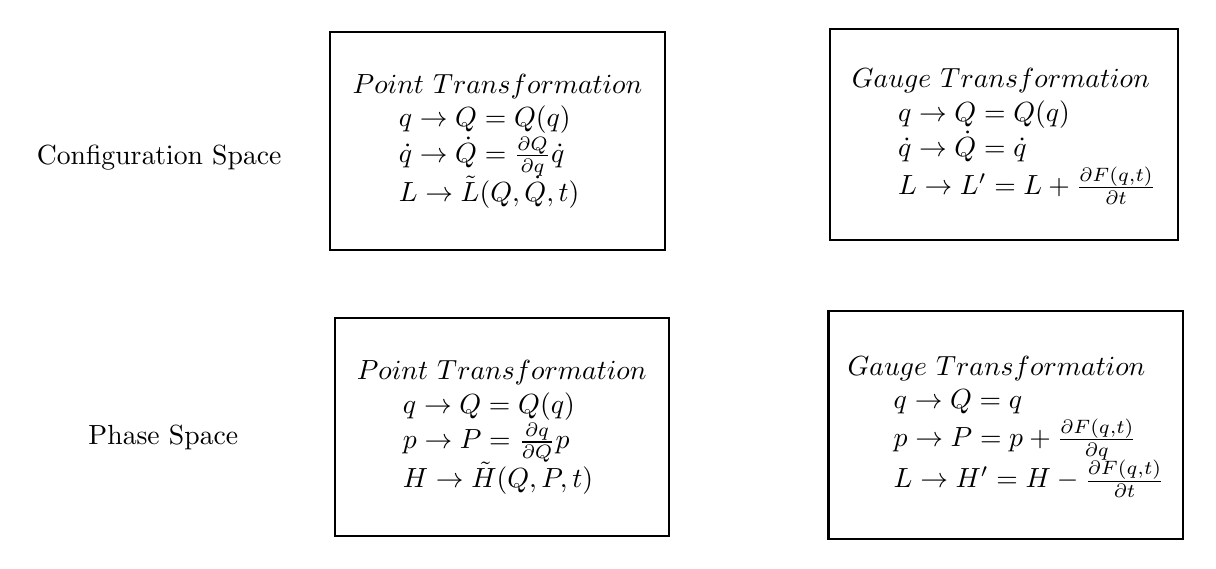
\begin{tikzpicture}[x=0.75pt,y=0.75pt,yscale=-1,xscale=1]
%uncomment if require: \path (0,300); %set diagram left start at 0, and has height of 300


% Text Node
\draw    (159.5,30.5) -- (320.5,30.5) -- (320.5,135.5) -- (159.5,135.5) -- cycle  ;
\draw (240,83) node    {$ \begin{array}{l}
Point\ Transformation\\
\ \ \ \ \ q\rightarrow Q=Q( q)\\
\ \ \ \ \ \dot{q}\rightarrow \dot{Q} =\frac{\partial Q}{\partial q}\dot{q}\\
\ \ \ \ \ L\rightarrow \tilde{L}( Q,\dot{Q} ,t)
\end{array}$};
% Text Node
\draw    (400,29) -- (568,29) -- (568,131) -- (400,131) -- cycle  ;
\draw (484,80) node    {$ \begin{array}{l}
Gauge\ Transformation\\
\ \ \ \ \ q\rightarrow Q=Q( q)\\
\ \ \ \ \ \dot{q}\rightarrow \dot{Q} =\dot{q}\\
\ \ \ \ \ L\rightarrow L^{\prime } =L+\frac{\partial F( q,t)}{\partial t}
\end{array}$};
% Text Node
\draw    (161.5,168.5) -- (322.5,168.5) -- (322.5,273.5) -- (161.5,273.5) -- cycle  ;
\draw (242,221) node    {$ \begin{array}{l}
Point\ Transformation\\
\ \ \ \ \ q\rightarrow Q=Q( q)\\
\ \ \ \ \ p\rightarrow P=\frac{\partial q}{\partial Q} p\\
\ \ \ \ \ H\rightarrow \tilde{H}( Q,P ,t)
\end{array}$};
% Text Node
\draw    (399.5,165) -- (570.5,165) -- (570.5,275) -- (399.5,275) -- cycle  ;
\draw (485,220) node    {$ \begin{array}{l}
Gauge\ Transformation\\
\ \ \ \ \ q\rightarrow Q=q\\
\ \ \ \ \ p\rightarrow P=p+\frac{\partial F( q,t)}{\partial q}\\
\ \ \ \ \ L\rightarrow H^{\prime } =H-\frac{\partial F( q,t)}{\partial t}
\end{array}$};
% Text Node
\draw (77,91) node   [align=left] {Configuration Space};
% Text Node
\draw (79,226) node   [align=left] {Phase Space};


\end{tikzpicture}

    \end{center}
\end{qt}

\subsection{Infinitesimal Canonical Transformation}
Mathematically, we can write a tiny transformation of our phase space coordinates as:
\begin{equation}
\begin{aligned}
&q_{i} \rightarrow Q_{i}=q_{i}+\epsilon D_{i}\left(q_{i}, p_{i}\right)\\
&p_{i} \rightarrow P_{i}=p_{i}+\epsilon E_{i}\left(q_{i}, p_{i}\right)
\end{aligned}
\label{infitrans}
\end{equation}
where $\epsilon$ is an infinitesimally small number. According to eqn.(\ref{poissonbracket}), we have
$$
\{Q, P\}_{q, p}=\frac{\partial Q}{\partial q} \frac{\partial P}{\partial p}-\frac{\partial Q}{\partial p} \frac{\partial P}{\partial q}
$$
$$
\begin{aligned}
&=1+\epsilon \frac{\partial D}{\partial q}+\epsilon \frac{\partial E}{\partial p}+\epsilon^{2} \frac{\partial D}{\partial q} \frac{\partial E}{\partial p}-\epsilon^{2} \frac{\partial D}{\partial p} \frac{\partial E}{\partial q}\\
&=1+\epsilon \frac{\partial D}{\partial q}+\epsilon \frac{\partial E}{\partial p}
\end{aligned}
$$
Thus,
\begin{equation}
    \frac{\partial D}{\partial q}+\frac{\partial E}{\partial p} \stackrel{!}{=} 0
\end{equation}

This implies that there must be a connection between $D$ and $E$. Specifically, we can conclude that the equation above is fulfilled if 
\begin{equation}
D=\frac{\partial G}{\partial p}, \quad \quad E=-\frac{\partial G}{\partial q}
\end{equation}
where $G=G(q, p)$ is some arbitrary function. Motivated by this observation, it is conventional to say that the new object $G$ generates the transformation. Moreover, \textbf{$G$ is called the generator of the canonical transformation.} The transformation in (\ref{infitrans}) therefore reads
\begin{qt}
    \begin{equation}
\begin{aligned}
&q_{i} \rightarrow Q_{i}=q_{i}+\epsilon \frac{\partial G}{\partial p}\\
&p_{i} \rightarrow P_{i}=p_{i}-\epsilon \frac{\partial G}{\partial q}
\end{aligned}
\label{infitrans2}
\end{equation}
\end{qt}
\bluep{The Poisson bracket is, in some sense, the natural product in phase space.} Therefore, if we consider an abstract phase space transformation:
$$
\begin{aligned}
q \rightarrow Q &=T \circ q, \quad p \rightarrow P=T \circ p \\
&=\{T, q\}, \quad=\{T, p\}
\end{aligned}
$$
Now \textbf{we let our generator $G$ act on the coordinates $q,p$ via the Poisson bracket.} To that end, we define an infinitesimal transformation as a linear combination of the identity transformation $I\circ X=X$ and the generator action:
$$
T_{\text {inf }} \circ X \equiv(I+\epsilon G) \circ X=X+\epsilon G \circ X
$$
We can then calculate:
$$
\begin{aligned}
q \rightarrow Q &=T_{\text {inf }} \circ q \\
&=q+\epsilon G \circ q \\
&=q+\epsilon\{q, G\}
&==q+\epsilon \frac{\partial G}{\partial p}
\end{aligned}
$$
Therefore, \textbf{our generator G really acts on the phase space coordinates via the Poisson bracket}. We can transform our phase space coordinates using any phase space function $G(q, p)$ We only have to make sure that $G$ acts on our coordinates via the appropriate phase space product, i.e., the Poisson bracket.

\subsection{Generating Functions}
In this section, we discover a new method to construct transformations between canonical coordinates systematically. We first write down the following transformation using a single function \redp{$F=F(q,Q,t)$} through the formulas:
\begin{qt}
    \begin{equation}
\begin{aligned}
&P=\frac{\partial F}{\partial Q}\\
&p=-\frac{\partial F}{\partial q}
\end{aligned}
\label{generattrans}
\end{equation}
\end{qt}
since $F$ is a function of $q, Q,$ and $t,$ we know that $\frac{\partial F}{\partial Q}$ will be a function of $q, Q,$ and $t$ too. Therefore, the second line in Eq. (\ref{generattrans}) is an equation of the form $p=p(q, Q, t) .$ We can then invert this equation to get an expression of the form \redp{$Q=Q(q, p, t) .$} So in other words, given some function $F,$ the second line tells us what our new location coordinates look like in terms of the original location and momentum coordinates. The first line yields a formula of the form $P=P(q, Q, t) .$ But we already know from the second line what $Q$ looks like in terms of the original coordinates. Therefore, we can use this expression to get a formula that specifies the new momentum coordinates $P$ solely in terms of the original phase space coordinates $P=P(q, p, t)$. Therefore, \redp{\textbf{Eq.(\ref{generattrans}) tells us everything that we need to know about how our old coordinates are related to the new ones.}}

As a concrete example, let’s calculate the canonical transformation generated by
\begin{equation}
F(q, Q)=q Q
\end{equation}
Using Eq.\ref{generattrans}, we find
\begin{equation}
\begin{aligned}
&P=\frac{\partial F}{\partial Q}=\frac{\partial(q Q)}{\partial Q}=q\\
&p=-\frac{\partial F}{\partial q}=-\frac{\partial(q Q)}{\partial q}=-Q
\end{aligned}
\end{equation}
This means that the canonical transformation generated by $F(q, Q)=q Q$ flips the roles of the momentum and location coordinates.

Hamilton’s equations follow as a condition on the path of least action for the Hamiltonian action
\begin{equation}
S=\int_{t_{\mathrm{i}}}^{t_{f}} L d t=\int_{t_{\mathrm{i}}}^{t_{f}}(p \dot{q}-H) d t
\end{equation}
where $L \equiv p \dot{q}-H$ is the \redp{"Hamiltonian Lagrangian"}. After the transformation $q, p \rightarrow Q, P$, the least action principle with an analogous Hamiltonian action
\begin{equation}
\tilde{S}=\int_{t_{\mathrm{i}}}^{t_{f}} L^{\prime} d t=\int_{t_{\mathrm{i}}}^{t_{f}} d t\left(P \dot{Q}-H^{\prime}\right)
\end{equation}
must still be valid, where $L^{\prime} \equiv P \dot{Q}-H^{\prime}$ is the transformed "Hamiltonian Lagrangian".

Because the transformation is based on a generating function, the original Lagrangian $L$ and the transformed Lagrangian differ by the total derivative of the generating function $F=F(q,Q,t)$:
\begin{qt}
    \begin{equation}
        L^{\prime}-L=\frac{d F}{d t}
    \end{equation}
\end{qt}
and
$$
\begin{aligned}
\frac{d F(q, Q)}{d t} &=\frac{\partial F}{\partial q} \frac{\partial q}{\partial t}+\frac{\partial F}{\partial Q} \frac{\partial Q}{\partial t}+\frac{\partial F}{\partial t} \\
&=\frac{\partial F}{\partial q} \dot{q}+\frac{\partial F}{\partial Q} Q+\frac{\partial F}{\partial t}
\end{aligned}
$$
With these two equations, we have
$$
\begin{array}{c}
{L^{\prime}-L=\frac{d F}{d t}} \\
{\left(P \dot{Q}-H^{\prime}\right)-(p \dot{q}-H)=\frac{\partial F}{\partial q} \dot{q}+\frac{\partial F}{\partial Q} \dot{Q}+\frac{\partial F}{\partial t}} \\
{\left(P-\frac{\partial F}{\partial Q}\right) \dot{Q}-\left(p+\frac{\partial F}{\partial q}\right) \dot{q}=H^{\prime}-H+\frac{\partial F}{\partial t}}
\end{array}
$$
None of the functions in last line depend explicitly on $\dot{q}$. Therefore, if we calculate the partial derivative with respect to $\dot{q}$, we find:
\begin{equation}
\begin{aligned}
\frac{\partial}{\partial \dot{q}}\left(P-\frac{\partial F}{\partial Q}\right) \dot{Q}-\frac{\partial}{\partial \dot{q}}\left(p+\frac{\partial F}{\partial q}\right) \dot{q} &=\frac{\partial}{\partial \dot{q}}\left(H^{\prime}-H+\frac{\partial F}{\partial t}\right) \\
-\left(p+\frac{\partial F}{\partial q}\right) &=0
\end{aligned}
\end{equation}
Similarly
\begin{equation}
\begin{aligned}
\frac{\partial}{\partial \dot{Q}}\left(P-\frac{\partial F}{\partial Q}\right) \dot{Q}-\frac{\partial}{\partial \dot{Q}}\left(p+\frac{\partial F}{\partial q}\right) \dot{q} &=\frac{\partial}{\partial \dot{Q}}\left(H^{\prime}-H+\frac{\partial F}{\partial t}\right) \\
\left(P-\frac{\partial F}{\partial Q}\right) &=0
\end{aligned}
\end{equation}
Therefore, we conclude:
$$
\begin{aligned}
&P=\frac{\partial F}{\partial Q}\\
&p=-\frac{\partial F}{\partial q}
\end{aligned}
$$
We can also calculate how the Hamiltonian gets modified by the canonical transformation generated by $F$ as:
\begin{qt}
    \begin{equation}
        H^{\prime}=H-\frac{\partial F}{\partial t}
        \label{generateHamil}
    \end{equation}
\end{qt}

The algorithm to produce a canonical transformation goes like this:
\begin{qt}
    \begin{itemize}
    \item Write down a specific generating function $F=F(q, Q, t)$
    \item Use Eq.\ref{generattrans} to find the formulas which express the new coordinates $(Q, P)$ in terms of the old ones $(q, p)$
    \item Use Eq.\ref{generateHamil} to caculate the new Hamiltonian $\tilde{H}(Q,P,t)$
\end{itemize}
\end{qt}

\section{The Harmonic Oscillator}
We call all systems with a potential of the form $V=c x^{2}$ where $c$ is some constant, a harmonic oscillator.